\part{Atmosphäre}

Neben den Wolken sollte auch die Atmosphäre dynamisch (hinsichtlich Umgebungsparameter) und physikalisch basiert, und
nicht bloß eine statische Skybox sein.

In diesem Abschnitt wird zunächst auf vorherige Arbeiten eingegangen, dann beschrieben, wie die Atmosphäre und
atmosphärische Effekte wie aerial perspective zustandekommen und akkurat modelliert werden können. Anschließend
werden die für Echtzeitrendendering nötigen Vereinfachungen und deren Einfluss auf das Modell erläutert und
die tatsächliche Umsetzung in Software umrissen, abschließend kurz die visuellen Ergebnisse und die erreichte
Performance betrachtet.

\section{Verwandte Arbeiten}
Da die Atmosphäre einen großen Teil vieler Szenen ausmacht, gibt es schon lange Modelle für das Rendern dieser.
Angefangen mit \cite{Nishita93}, in dem das hier verwendete Modell seinen Ursprung hat, gefolgt von
\cite{Schafhitzel07}, die die Dimensionen Höhe, Sonnenwinkel, Blickwinkel für die primäre Streuungstextur einführen.
In \cite{Bruneton08} wird die Parametrisierung der LUT verbessert, die Idee die Auswertung der Phase Function zu
verzögern stammt von \cite{Elek09}.

Die Hauptquelle für dieses Projekt ist allerdings \cite{Bodare14}, unsere Atmosphäre ist direkt nach den dort
vorgestellten Algorithmen und Ideen (dynamische Atmosphäre) implementiert.

\section{Modell}

Um die Atmosphäre zu rendern muss zunächst verstanden werden, wie unsere Wahrnehmung dieser überhaupt zustande kommt.
Anschließend werden diese Erkenntnisse physikalisch realisiert und schließlich ein mathematisches Modell für die
verschiedenen Phänomene die das Aussehen der Atmosphäre bestimmen erschlossen. Dann wird auf die Implementierung
eingegangen, und abschließend der Realismus und die Performance evaluiert.

\subsection{Überblick}
Die Atmosphäre besteht aus Partikeln die Licht sowohl streuen als auch dämpfen.

Schaut man in den Himmel sieht man nicht diese mikroskopisch kleinen Partikel, sondern das Licht, welches von diesen in
das Auge gestreut wird. Das gestreute Licht stammt entweder direkt von einer Lichtquelle (der Sonne oder anderen
Himmelskörpern, oder sogar von welchen an der Erdoberfläche), oder wurde bereits von einem anderen Partikel gestreut. In
ersterem Fall spricht man von Einfacher- in letzterem von Mehrfacher Streuung. Die Stärke der Streuung hängt neben der
Art der Partikel auch von der Wellenlänge des einfallenden Lichtes ab, was die Farbunterschiede zu verschiedenen
Sonnenständen erklärt (je nach Sonnenstand streuen andere und unterschiedlich viele Partikel das direkte Sonnenlicht,
welches den Hauptteil des einfallenden Lichtes, und damit der Farbe des Himmels, ausmacht).

Wie bereits erwähnt streuen die Partikel nicht nur, sie dämpfen das gestreute (oder direkte!) Licht auch. Der Grund für
diese Dämpfung ist zum einen, dass Licht nicht nur in das Auge hinein, sondern auch aus dem direkten Pfad zum Auge
herausgestreut wird, und zum anderen, dass Partikel wie Ozon einen Teil des Lichtes auf dem Weg zum Auge absorbieren.

Neben der Farbe des Himmel erklären Streuung und Dämpfung auch, warum weit entfernte Gebirgsketten eine Farbänderung
erfahren: zum einen streuen Partikel zwischen Auge und Objekt Licht verschiedener Wellenlängen in den direkten Pfad
zwischen Auge und Objekt, und zum anderen streuen sie von dem Objekt reflektiertes Licht aus diesem Pfad heraus, so dass
es nicht in das Auge gelangt (Die Farbe des Objektes wird gedämpft und geht durch Streuung auf dem Pfad zwischen Auge
und Objekt in die Farbe des Himmels über).

\begin{figure}[h]
	\centering
	\begin{tikzpicture}
	\useasboundingbox (0.0) rectangle (8.4,4.9);
	\begin{scope}[transform canvas={scale=0.7}]
	\clip (0,0) rectangle (12,7);
	\filldraw[fill=blue!20] (1, -10) circle (16);
	\filldraw[fill=green!20] (1, -10) circle (11);

	\path[name path=atmosphere] (1, -10) circle (16);

	\coordinate (eye) at (1, 2);
	\centerarc[thick](eye)(20:-10:.4);
	\draw[] (eye) -- ($(eye) + .5*({cos(20)}, {sin(20)})$);
	\draw[] (eye) -- ($(eye) + .5*({cos(-10)}, {sin(-10)})$);
	\path[name path=view] (eye) -- ($(eye) + 10*({cos(5)}, {sin(5)})$);

	\path[name path=eye_c1] (eye) circle (.55);

	\path[name path=eye_c2] (eye) circle (1.7);
	\path[name path=eye_forw1] (eye) -- ($(eye) + 10*({cos(13)}, {sin(13)})$);
	\node[name intersections={of=eye_c1 and eye_forw1}] (eye_c1_i1) at (intersection-1) {};
	\node[name intersections={of=eye_c2 and eye_forw1}] (eye_c2_i1) at (intersection-1) {};

	\path[name path=eye_c3] (eye) circle (3.5);
	\path[name path=eye_forw2] (eye) -- ($(eye) + 10*({cos(0)}, {sin(0)})$);
	\node[name intersections={of=eye_c1 and eye_forw2}] (eye_c1_i2) at (intersection-1) {};
	\node[name intersections={of=eye_c3 and eye_forw2}] (eye_c3_i1) at (intersection-1) {};

	\path[name path=eye_c4] (eye) circle (5);
	\path[name path=eye_forw3] (eye) -- ($(eye) + 10*({cos(-9)}, {sin(-9)})$);
	\node[name intersections={of=eye_c1 and eye_forw3}] (eye_c1_i3) at (intersection-1) {};
	\node[name intersections={of=eye_c4 and eye_forw3}] (eye_c4_i1) at (intersection-1) {};

	% \coordinate(pb) at (intersection 1 of atmosphere and view);

	\coordinate (p1) at (3.8, 4);
	\path[name path=pp1] (p1) -- ($(p1) + 10*({cos(40)}, {sin(40)})$);
	\draw[->, dashed, name intersections={of=atmosphere and pp1}]
		(intersection-1) --
		(p1) --
		(eye_c2_i1.center) --
		(eye_c1_i1.center);

	\path[name path=pp2] (eye_c3_i1.center) -- ($(eye_c3_i1.center) + 10*({cos(40)}, {sin(40)})$);
	\draw[->, dashed, name intersections={of=atmosphere and pp2}]
		(intersection-1) --
		(eye_c3_i1.center) --
		(eye_c1_i2.center);

	\coordinate (out_mid) at ($(eye_c4_i1.center)!.8!(eye_c1_i3.center)$);
	\path[name path=pp3] (eye_c4_i1.center) -- ($(eye_c4_i1.center) + 10*({cos(40)}, {sin(40)})$);
	\draw[->, dashed, name intersections={of=atmosphere and pp3}]
		(intersection-1) --
		(eye_c4_i1.center) --
		(out_mid) -- (.5, 1.6);

	\coordinate (l2) at ($(1, -10) + 16.5*({cos(73)}, {sin(73)})$);
	\draw[thick, <-, yellow!80!orange] (l2) -- ++($({cos(40)}, {sin(40)})$);
	
	\coordinate (l1) at ($(1, -10) + 16.5*({cos(69)}, {sin(69)})$);
	\draw[thick, <-, yellow!80!orange] (l1) -- ++($({cos(40)}, {sin(40)})$);
	
	\coordinate (l3) at ($(1, -10) + 16.5*({cos(64)}, {sin(64)})$);
	\draw[thick, <-, yellow!80!orange] (l3) -- ++($({cos(40)}, {sin(40)})$);
	
	\coordinate (l4) at ($(1, -10) + 16.5*({cos(59)}, {sin(59)})$);
	\draw[thick, <-, yellow!80!orange] (l4) -- ++($({cos(40)}, {sin(40)})$);
	
	\coordinate (l5) at ($(1, -10) + 16.5*({cos(56)}, {sin(56)})$);
	\draw[thick, <-, yellow!80!orange] (l5) -- ++($({cos(40)}, {sin(40)})$);

	\end{scope}
	\end{tikzpicture}
	\caption{Mehrfache-, Einfache- und Ausstreuung}
	\label{streuung}
\end{figure}

\begin{figure}[h]
	{\centering
	\begin{tikzpicture}
	\useasboundingbox (0.0) rectangle (8.4,4.9);
	\begin{scope}[transform canvas={scale=0.7}]
	\fill[fill=blue!20] (0,0) rectangle (12,7);
	\fill[fill=green!20] (0,0) rectangle (12,1);

	\coordinate (eye) at (1, 2);
	\centerarc[thick](eye)(20:-10:.4);
	\draw[] (eye) -- ($(eye) + .5*({cos(20)}, {sin(20)})$);
	\draw[] (eye) -- ($(eye) + .5*({cos(-10)}, {sin(-10)})$);
	\coordinate (eye_to) at ($(eye) + 10*({cos(10)}, {sin(10)})$);
	\path[name path=view] (eye) -- (eye_to);

	\path[name path=tri, fill=red] (8,1) -- (9.5,5) -- (11,1) -- cycle;

	\draw[dashed, red] ($(eye)!0.79!(eye_to)$) -- ($(eye)!0.70!(eye_to)$);
	\draw[dashed, orange] ($(eye)!0.71!(eye_to)$) -- ($(eye)!0.40!(eye_to)$);
	\draw[dashed, orange!70!blue] ($(eye)!0.395!(eye_to)$) -- ($(eye)!0.25!(eye_to)$);
	\draw[->, dashed, orange!60!blue] ($(eye)!0.25!(eye_to)$) -- ($(eye)!0.05!(eye_to)$);

	\coordinate (p1) at ($(eye)!0.70!(eye_to)$);
	\draw[->, dashed, yellow] ($(p1) + 2*({cos(55)}, {sin(55)})$) -- (p1);
	\node[below=1mm of p1] {$p_1$};

	\coordinate (p2) at ($(eye)!0.40!(eye_to)$);
	\draw[->, dashed, blue] ($(p2) + ({cos(320)}, {sin(320)})$) -- (p2);
	\node[below=1mm of p2] {$p_2$};

	\coordinate (p3) at ($(eye)!0.25!(eye_to)$);
	\draw[<-, dashed, orange!70!blue] ($(p3) + ({cos(170)}, {sin(170)})$) -- (p3);
	\node[below=1mm of p3] {$p_3$};

	\end{scope}
	\end{tikzpicture}
	}
	
	Bei $p_1$ wird ein Sonnenstrahl in die Blickrichtung gestreut, bei $p_2$ ein bereits gestreuter Lichstrahl aus der
	Atmosphäre. $p_3$ zeigt die Transmittance (Ausstreuung, Absorption durch Beispielsweise Ozon ist nicht abgebildet).

	Die Farbänderungen sind eher symbolisch als realistisch.
\caption{Aerial Perspective}
\label{AP}
\end{figure}

\subsection{Physikalische Basis}

Um das Streuverhalten der Partikel in der Atmosphäre anzunähern werden Mie- und Rayleigh-Streuung verwendet. Bei
Partikeln mit
\begin{equation}
	d \ll \frac{\lambda}{2\pi}
\end{equation}
(z.B. Luftmolekülen), wobei $d$ Durchmesser und $\lambda$ die Wellenlänge des gestreuten Lichtes ist, wird die Streuung
mit Rayleigh, bei Partikel mit größerem Durchmesser (Staub, Eis, Wassertropfen) mit Mie angenähert. Ein Unterschied
zwischen Mie- und Rayleigh-Streuung ist, dass bei Rayleigh die Intensität des gestreuten Lichtes von der Wellenlänge des
einfallenden Lichtes abhängt, während Mie (in diesem Modell) unabhängig von dieser streut.

Die Absorption durch Ozon ist ebenfalls Wellenlängenabhängig: manche Wellenlängen werden stärker, andere schwächer
absorbiert. Dadurch wird erneut die Farbe des einfallenden Lichtes beeinflusst.

\subsection{Mathematisches Modell}
\begin{table}
	\centering
	\begin{tabular}{| c | c |}
	\hline
	Symbol & Definition\\ \hline
	$I_I$ & Intensität des einfallenden Lichtes\\
	$\beta_{R,M}$ & Rayleigh/Mie scattering coefficient\\
	$\beta^e_{R,M,O}$ & Rayleigh/Mie/Ozone extinction coefficient\\
	$F_{R,M}$ & Rayleigh/Mie phase function\\
	$\rho_{R,M,O}$ & Rayleigh/Mie/Ozone density function\\
	$v$ & Blickrichtung\\
	$l$ & Lichtquellenrichtung\\
	$p$ & Position\\
	$\lambda$ & Wellenlänge\\ \hline
	\end{tabular}
	\caption{Verwendete Symbole}
	\label{symbols}
\end{table}

Aus den Ergebnissen der physikalischen Betrachtung lassen sich für das Rendern notwendige Formeln ableiten.

Das Ziel ist, die Atmosphäre akkurat zu renderen, also die gesamte Intensität $1,2, \dots k$-fach Mie und Rayleigh
gestreuten Lichtes einer Wellenlänge $\lambda$ für einen Augpunkt $p$, eine Blickrichtung $v$ und eine
Lichtquellenrichtung $l$ zu berechnen.

Im Folgenden wird angenommen, dass einerseits lediglich die Sonne Licht in die Atmosphäre beisteuert und andererseits
alle Strahlen dieser als Parallel betrachtet werden können (was hinsichtlich der relativen Intensität und Entfernung
dieser das Modell nicht erwähnenswert beeinträchtigt).

Um die Intensität mehrfach gestreuten Lichtes zu bestimmen, ist es sinnvoll, das Problem auf die einfachere Bestimmen
der Intensität einfach gestreuten Lichtes zu reduzieren. Dafür wird zunächst die einzelne Mie/Rayleigh-Streuung
modelliert:
\begin{equation}
	I_{S_{R,M}}(p, o, i, \lambda) = \frac{I_I(\lambda)\rho_{R,M}(p)F_{R,M}(\theta)\beta_{R,M}(\lambda)}{4\pi}
\end{equation}
wobei $i$ die Richtung des einfallenden, $o$ die Richtung des gestreuten Lichtes und $\theta$ der Winkel zwischen $i$
und $o$ ist. Die Intensität gestreuten Lichtes hängt neben Wellenlänge ($\beta_{R,M}(\lambda)$) und Winkel zwischen ein-
und ausfallendem Licht ($F_{R,M}(\theta)$) auch von der lokalen Partikeldichte ($\rho_{R,M}(p)$) ab. Die in diesem
Modell dafür verwendeten Gleichungen werden in \cref{formeln} erläutert.

Das gesamte durch einfache Rayleigh- oder Mie-Streuung einfallende Licht an einem Punkt $p_a$ wird mit dem Integral über
alle einzelnen Streuungen entlang $v$ (bis zum Rand der Atmosphäre), die in Richtung $-v$ streuen bestimmt (siehe
\cref{SS-image}). Da sich das Licht dabei durch die Atmosphäre bewegt, muss die dämpfende Transmittance
\begin{equation}
	T(p_a, p_b, \lambda) = \exp\bigg(-\sum_{i\in R,M,O}^{} \beta^e_i(\lambda) \int_{p_a}^{p_b} \rho_i(p) \,dp\bigg)
\end{equation}
beachtet werden.

Da die Richtung in welche das aus dem Sichtstrahl gestreute Licht gestreut wird egal ist (nur \textit{wieviel} überhaupt
gestreut wird ist relevant) fällt die phase function aus dem Streuungsterm heraus. Neben Streuung modelliert
$\beta^e_{M,O}$ (ohne $\beta^e_R$ da die durch Rayleigh modellierten Moleküle nur streuen) auch Absorption. Da beide
mit Partikeldichte skalieren ist es sinnvoll sie in einen Term zu kombinieren.

\begin{equation}\label{eq:ss}
	\begin{aligned}
		I^{(1)}_{R,M}(p_a,v,l,\lambda) = \int_{p_a}^{p_b} &T(p_l, p, \lambda)T(p, p_a, \lambda) \\
		&I_{S_{R,M}}(p, -v, -l, \lambda) \,dp\\
	\end{aligned}
\end{equation}

$p_l$ ist der Schnittpunkt von einem Strahl $p+t \cdot l$ mit der Atmosphäre. Dieser Schnittpunkt ist interessant, weil
das Licht zunächst auf $p_l \rightarrow p$ und dann auf $p \rightarrow p_a$ gedämpft wird, bis es schließlich bei $p_a$
in das Auge fällt (siehe \cref{SS-image}).

\begin{figure}[h]
	\centering
	\begin{tikzpicture}
	\useasboundingbox (0.0) rectangle (8.4,4.9);
	\begin{scope}[transform canvas={scale=0.7}]
	\clip (0,0) rectangle (12,7);
	\filldraw[fill=blue!20] (1, -10) circle (16);
	\filldraw[fill=green!20] (1, -10) circle (11);

	\path[name path=atmosphere] (1, -10) circle (16);

	\coordinate (eye) at (1, 2);
	\centerarc[thick](eye)(20:-10:.4);
	\draw[] (eye) -- ($(eye) + .5*({cos(20)}, {sin(20)})$);
	\draw[] (eye) -- ($(eye) + .5*({cos(-10)}, {sin(-10)})$);
	\path[name path=view] (eye) -- ($(eye) + 10*({cos(5)}, {sin(5)})$);

	% \coordinate(pb) at (intersection 1 of atmosphere and view);

	% \node[name intersections={of=atmospherea and view}] (intersection) {$p_b$};
	\node[red, name intersections={of=atmosphere and view}] (pb) at (intersection-1) {};
	\node[below=0 of pb.center] {$p_b$};
	\draw[<-, dashed] ($(eye) + .5*({cos(5)}, {sin(5)})$) -- (pb.center);

	\coordinate (p1) at ($(eye)!0.2!(pb)$);
	\node[below=0 of eye.center] {$p_a$};

	\path[name path=sun1] (p1) -- ($(p1) + 10*({cos(40)}, {sin(40)})$);
	\node[red, name intersections={of=atmosphere and sun1}] (pl1) at (intersection-1) {};
	\node[below=0 of p1.center] {$p_{1}$};
	\draw[dashed] (p1) -- (pl1.center);
	\node[below=1mm of pl1.center] {$p_{l1}$};

	\coordinate (p2) at ($(eye)!0.35!(pb)$);
	\path[name path=sun2] (p2) -- ($(p2) + 20*({cos(40)}, {sin(40)})$);
	\node[red, name intersections={of=atmosphere and sun2}] (pl2) at (intersection-1) {};
	\node[below=0 of p2.center] {$p_{2}$};
	\draw[dashed] (p2) -- (pl2.center);
	\node[below=1mm of pl2.center] {$p_{l2}$};

	\coordinate (p3) at ($(eye)!0.7!(pb)$);
	\path[name path=sun3] (p3) -- ($(p3) + 30*({cos(40)}, {sin(40)})$);
	\node[below=0 of p3.center] {$p_{3}$};
	\node[red, name intersections={of=atmosphere and sun3}] (pl3) at (intersection-1) {};
	\draw[dashed] (p3) -- (pl3.center);
	\node[below=1mm of pl3.center] {$p_{l3}$};

	\coordinate (l2) at ($(1, -10) + 16.5*({cos(73)}, {sin(73)})$);
	\draw[thick, <-, yellow!80!orange] (l2) -- ++($({cos(40)}, {sin(40)})$);

	\coordinate (l1) at ($(1, -10) + 16.5*({cos(69)}, {sin(69)})$);
	\draw[thick, <-, yellow!80!orange] (l1) -- ++($({cos(40)}, {sin(40)})$);

	\coordinate (l3) at ($(1, -10) + 16.5*({cos(64)}, {sin(64)})$);
	\draw[thick, <-, yellow!80!orange] (l3) -- ++($({cos(40)}, {sin(40)})$);

	\coordinate (l4) at ($(1, -10) + 16.5*({cos(59)}, {sin(59)})$);
	\draw[thick, <-, yellow!80!orange] (l4) -- ++($({cos(40)}, {sin(40)})$);

	\coordinate (l5) at ($(1, -10) + 16.5*({cos(56)}, {sin(56)})$);
	\draw[thick, <-, yellow!80!orange] (l5) -- ++($({cos(40)}, {sin(40)})$);

	\end{scope}
	\end{tikzpicture}
	\caption{Einfache Streuung für drei $p$: $p_1, p_2, p_3$}
	\label{SS-image}
\end{figure}

Das Berechnen der Irradianz des $k$-fach gestreuten Lichtes wird in zwei Schritte aufgeteilt:

Im Ersten, im Folgenden \emph{Gathering}, wird die Irradianz des in einem Punkt $p$ einfallenden und in eine Richtung $o$
ausfallendem, $k-1$-fach gestreuten Lichtes bestimmt ($\theta$ ist wieder der Winkel in dem gestreut wird, also
$\angle(o, -l)$).

\begin{equation} \label{eq:g}
	G^{(k)}_{R,M}(p,o,l,\lambda) = \int_{4\pi}^{} F_{R,M}(\theta)I^{(k)}_{R,M}(p,\omega,l,\lambda) \,d\omega
\end{equation}


Im Zweiten wird dieses Gathering entlang eines Sichtstrahls integriert:

\begin{equation} \label{eq:ms}
	\begin{aligned}
		I^{(k)}_{S_{R,M}}(p_a, v, l, \lambda) = \frac{\beta_{R,M}(\lambda)}{4\pi} &\int_{p_a}^{p_b}
		G^{(k-1)}_{R,M}(p,-v,l,\lambda)\\ &\rho_{R,M}(p) T(p, p_a, \lambda) \,dp
	\end{aligned}
\end{equation}

\begin{figure}
	\centering
	\begin{tikzpicture}
	\useasboundingbox (0.0) rectangle (8.4,4.9);
	\begin{scope}[transform canvas={scale=0.7}]
	\clip (0,0) rectangle (12,7);
	\filldraw[fill=blue!20] (1, -10) circle (16);
	\filldraw[fill=green!20] (1, -10) circle (11);

	\path[name path=atmosphere] (1, -10) circle (16);

	\coordinate (eye) at (1, 2);
	\centerarc[thick](eye)(20:-10:.4);
	\draw[] (eye) -- ($(eye) + .5*({cos(20)}, {sin(20)})$);
	\draw[] (eye) -- ($(eye) + .5*({cos(-10)}, {sin(-10)})$);
	\path[name path=view] (eye) -- ($(eye) + 10*({cos(5)}, {sin(5)})$);

	% \coordinate(pb) at (intersection 1 of atmosphere and view);

	% \node[name intersections={of=atmospherea and view}] (intersection) {$p_b$};
	\node[red, name intersections={of=atmosphere and view}] (pb) at (intersection-1) {};
	\node[below=0 of pb.center] {$p_b$};
	\draw[dashed, <-] ($(eye) + .5*({cos(5)}, {sin(5)})$) -- (pb.center);
	\node[below=0 of eye.center] {$p_a$};

	\node[circle, minimum size=.15cm, inner sep=0] (p1) at ($(eye)!0.2!(pb)$) {};
	\node[minimum size=1cm, circle, label=below:$p_1$] (c1) at (p1) {};
	\draw[->, dashed] (c1.72) -- (p1.72);
	\draw[->, dashed] (c1.0) -- (p1.0);
	\draw[->, dashed] (c1.144) -- (p1.144);
	\draw[->, dashed] (c1.216) -- (p1.216);
	\draw[->, dashed] (c1.288) -- (p1.288);

	\node[circle, minimum size=.15cm, inner sep=0] (p2) at ($(eye)!0.35!(pb)$) {};
	\node[minimum size=1cm, circle, label=below:$p_2$] (c2) at (p2) {};
	\draw[->, dashed] (c2.97) -- (p2.97);
	\draw[->, dashed] (c2.25) -- (p2.25);
	\draw[->, dashed] (c2.169) -- (p2.169);
	\draw[->, dashed] (c2.241) -- (p2.241);
	\draw[->, dashed] (c2.313) -- (p2.313);

	\node[circle, minimum size=.15cm, inner sep=0] (p3) at ($(eye)!0.7!(pb)$) {};
	\node[minimum size=1cm, circle, label=below:$p_3$] (c3) at (p3) {};
	\draw[->, dashed] (c3.121) -- (p3.121);
	\draw[->, dashed] (c3.49) -- (p3.49);
	\draw[->, dashed] (c3.193) -- (p3.193);
	\draw[->, dashed] (c3.265) -- (p3.265);
	\draw[->, dashed] (c3.337) -- (p3.337);

	\coordinate (l2) at ($(1, -10) + 16.5*({cos(73)}, {sin(73)})$);
	\draw[thick, <-, yellow!80!orange] (l2) -- ++($({cos(40)}, {sin(40)})$);

	\coordinate (l1) at ($(1, -10) + 16.5*({cos(69)}, {sin(69)})$);
	\draw[thick, <-, yellow!80!orange] (l1) -- ++($({cos(40)}, {sin(40)})$);

	\coordinate (l3) at ($(1, -10) + 16.5*({cos(64)}, {sin(64)})$);
	\draw[thick, <-, yellow!80!orange] (l3) -- ++($({cos(40)}, {sin(40)})$);

	\coordinate (l4) at ($(1, -10) + 16.5*({cos(59)}, {sin(59)})$);
	\draw[thick, <-, yellow!80!orange] (l4) -- ++($({cos(40)}, {sin(40)})$);

	\coordinate (l5) at ($(1, -10) + 16.5*({cos(56)}, {sin(56)})$);
	\draw[thick, <-, yellow!80!orange] (l5) -- ++($({cos(40)}, {sin(40)})$);

	\end{scope}
	\end{tikzpicture}
	\caption{Mehrfache Streuung und Gathering für drei $p$: $p_1, p_2, p_3$}
	\label{MS-image}
\end{figure}

(Hier sei kurz erwähnt, dass $k-1$-Gathering und $k$-Scattering sehr eng zusammengehören; sie modellieren gemeinsam eine
Streuung. Die Aufteilung von $F,\rho,$ und $\beta$ auf die beiden Formeln ist ziemlich arbritär, hier wird nur das
nötigste, also $F$ in Gathering belassen. Die beiden Formeln werden überhaupt aufgeteilt, weil das separate Gathering
später die Effizienz der Implementierung erhöht).

Um die gesamte Intensität des aus der Atmosphäre einfallenden Lichtes mit bis zu $K$ Streuungen zu bestimmen, muss die
Intensität von Rayleigh- und Mie-Streuung für jede Streuungsordnung $i \le K$ aufsummiert werden:

\begin{equation} \label{eq:insc_total}
	I_S(p,v,l,\lambda) = \sum^{K}_{i=1} I^{(i)}_{S_R}(p, v, l, \lambda) + I^{(i)}_{S_M}(p, v, l, \lambda) 
\end{equation}

\subsection{Dynamische Atmosphäre}
Neben der Atmosphäre sollten insbesondere auch Wetteränderungen realistisch dargestellt werden. Das wird hier durch
einfaches Überblenden erreicht, also wird das Aussehen der alten Atmosphäre für einen kurzen Zeitraum mit dem der Neuen
vermischt, bis nur noch die Neue sichtbar ist.

\subsection{Ground Lighting}
Das Umgebungslicht, das für einen gegebenen Punkt an der Erdoberfläche ankommt kann mit
\begin{equation} \label{eq:gl}
	I_A(p,l,\lambda) = \int_{2\pi}^{} (n \bullet \omega)I_S(p, \omega, l, \lambda) \,d\omega
\end{equation}
bestimmt werden. $n$ ist die Normale an dem Punkt $p$.

\subsection{Direktes Sonnenlicht}
Das Direkte Sonnenlicht wird mit
\begin{equation*}
	I^{(0)}_S(p,l,\lambda) = I_I(\lambda)T(p_a, p_b)
\end{equation*}
bestimmt, $p_b$ ist dabei der Schnittpunkt des Sonnenlichts mit der Atmosphäre.

\section{Implementierung}

\begin{table}[h]
	\centering
	\begin{tabular}{| c | p{15em} |}
	\hline
	Symbol & Definition \\ \hline
	$K$ & Anzahl zu berechnender Streuungsordnungen\\
	$s_{x,y,z}$ & Blickwinkel-, Höhen-, Sonnenwinkel-Auflösung der Streuungstextur\\
	$ap_{x,y,z}$ & $x,y,z$-Auflösung der Streuungstextur\\ \hline
	\end{tabular}
	\caption{Verwendete Symbole}
	\label{symbols}
\end{table}

Da für uns die Echtzeitgrafik, nicht hochpräzise Simulation, im Vordergrund steht, wird die Atmosphäre vorberechnet,
sodass zur Laufzeit (bestenfalls) nur noch eine Textur ausgelesen werden muss.

Im folgenden werden zunächst Anpassungen des Modells erläutert, dann wird das verwendete System skizziert und schließlich auf
verschiedene Optimierungen eingegangen.

\subsection{Anpassungen des Modells für Echtzeitrendering}
\begin{figure}[h]
\begin{mdframed}
\begin{itemize}
\item 2 Dimensionen für die Richtung der Lichtquelle (Azimuth- und Zenithwinkel)
\item 3 Dimensionen für die Position des Betrachters (Höhe, Azimuth-, Zenithwinkel)
\item 2 Dimensionen für die Blickrichtung (Azimuth- und Zenithwinkel)
\end{itemize}
\end{mdframed}
\caption{Parameter des vollständigen Modells}
\label{params:full}
\end{figure}

Das Vorberechnen, dessen Vorteile bereits erläutert wurden, hat die Nachteile, dass sowohl Speicherbedarf als auch
Vorberechenzeit für das Modell in seiner aktuellen Form (7-Dimensional, siehe \cref{params:full})
unverhältnismäßig (im Vergleich zu anderen Systemen die zu dem Realismus einer gerenderten Szene beitragen) hoch sind.

Hier wurden folgende Annahmen getroffen um die Parameter der Vorberechnung von 7 Dimensionen auf lediglich 3 zu reduzieren:

\begin{enumerate}
	\item Die Erde ist eine perfekte Kugel
	\item $\rho_{R,M,O}$ hängen nur von der Höhe ab
	\item Lichtstrahlen, welche die Atmosphäre erreichen, sind exakt parallel
	\item Die Azimuth-Differenz zwischen Blick- und Lichtquellenwinkel kann ignoriert und stattdessen durch eine
	modifizierte Rayleigh phase function modelliert werden: $F_R(\theta) = \frac{8}{10}(\frac{7}{5}+\frac{1}{2}\cos(\theta))$
\end{enumerate}

(Annahmen 1-3 haben ihren Ursprung in \cite{Bruneton08}, Annahme 4 stammt von \cite{Elek09})

Durch das Ignorieren der Azimuth-Differenz geht die (wegen Mehrfacher Streuung ohnehin nicht besonders sichtbare)
Schattierung der Atmosphäre durch die Erde verloren. Außerdem würde ohne die Azimuth-Differenz die Atmosphäre in allen
Horizontalen Blickrichtungen gleich aussehen, dies kann aber mit einem verzögerten Auswerten (während des Renderns) der
phase functions $F_{R,M}$ verhindert werden. Ein positiver Nebeneffekt davon ist auch, dass die stark
Blick-Sonnenwinkelabhängige Mie-Streuung nicht von der Auflösung der Atmosphären-LUTs abhängig ist, und somit sehr fein
bestimmt werden kann ohne den Speicherbedarf in die Höhe zu treiben.


\subsection{Atmospäre}

Um die Atmosphäre vorzuberechnen muss die an einem Augpunkt für einen gegebenen Blick- und Sonnenwinkel einfallended
Irradianz für die (der einfachheit halber) Wellenlängen von Rotem (650nm), Grünem (510nm) und Blauem (475nm) Licht
gespeichert werden. Es muss also \cref{eq:insc_total} wiederholt ausgewertet werden. Für die Berechnung der Integrale
wird hier die Trapezregel mit festen Schrittlängen angewandt (alternativ auch mit fester Schrittzahl, wie in
\cite{Bodare14}). Die rekursiven Integrale (zum Beispiel bei Mehrfacher Streuung, \cref{eq:ms}) werden mit einem
iterativen Verfahren gelöst: zuerst wird der LUT für Einfache Streuung berechnet, dann der für einfaches Gathering, und
mit diesem wiederum die zweifache Streuung, zweifaches Gathering, dreifache Streuung, bis die gewünschte Anzahl an
maximalen Streuungen erreicht ist. Neben der Streuung wird auch das Gathering aufsummiert und gespeichert, da mit diesem
Mehrfache Streuung in die Berechnung der Aerial Perspective einbezogen wird. Das gesamte Verfahren (inklusive aerial
perspective und Transmittance-Vorberechnung) ist in \cref{precomp} skizziert.

Die Atmosphäre wird auf die Far Plane gezeichnet. Die einem Fragment entsprechende Blickrichtung kann im Vertex Shader
mit inverser Projektion berechnet werden und wird interpoliert an den Fragment Shader gegeben. Hier kann mit Höhe,
Blick- und Sonnenwinkel die für die Wellenlängen von RGB gespeicherte Streuung ausgelesen und die Phase Function auf
diese angewandt werden, was die Intensität der Atmosphäre für die jeweilige Wellenlänge und dieses Fragment ergibt.

\begin{figure}[H]
	\hspace{-6em}
	\begin{tikzpicture}[
	every node/.style={inner sep=8, rounded corners=1},
	node distance = 1,
	T_p/.style={rectangle, draw=blue, fill=white, thick},
	T_t/.style={rectangle, draw=blue, fill=blue!5, thick},
	SS_p/.style={rectangle, draw=red, fill=white, thick},
	S_t/.style={rectangle, draw=red, fill=red!5, thick},
	MS_p/.style={rectangle, draw=orange, fill=white, thick},
	G_p/.style={rectangle, draw=yellow, fill=white, thick},
	G_t/.style={rectangle, draw=yellow, fill=yellow!5, thick},
	R_p/.style={rectangle, draw=gray, fill=white, thick}
	]
	\begin{scope}[transform canvas={scale=0.7}]

	\matrix[column sep=1cm, row sep=1cm] (m) {
	& \node[T_p] (T) {Transmittance}; & \\
	& \node[SS_p] (SS) {Einfache Streuung}; & \\
	& \node[G_p] (G) {Gathering}; & \node[MS_p] (MS) {Mehrfache Streuung}; \\
	\node[T_t] (TT) {Transmittance}; & \node[G_t] (GT) {Gesamtes Gathering}; & \node[S_t] (S) {Gesamte Streuung}; \\
	& & \node[R_p] (A) {Atmosphäre}; \\
	& \node[R_p] (Pp) {AP-Vorberechnung}; & \node[R_p] (P) {Aerial Perspective}; \\
	};

	\node[
		draw,
		thick,
		inner ysep=.5cm,
		yshift=-.05cm,
		fit=(G) (MS),
		rounded corners=0,
		label={[label distance=-.68cm]90:$K-1$-mal}] (box1) {};
	\node[
		draw,
		dashed,
		inner ysep=.5cm,
		yshift=-.05cm,
		fit=(A) (P) (Pp),
		rounded corners=0,
		label={[label distance=-.71cm]270:Rendering}] (box2) {};
	\node[
		draw,
		dashed,
		inner ysep=.75cm,
		yshift=-.05cm,
		inner xsep=.4cm,
		xshift=.15cm,
		fit=(T) (SS) (G) (MS),
		rounded corners=0,
		label={[label distance=-.71cm]90:Vorberechnung}] (box3) {};

	\draw[->] (T.west) -| ($(TT.north)-(.3,0)$);
	\draw[->] ($(TT.north)-(.1,0)$) |- ($(MS.north) + (0,2.4)$) -- (MS.north);
	\draw[->] ($(TT.north)+(.1,0)$) |- (SS.west);
	\draw[->] ($(TT.north)+(.3,0)$) |- (G.west);
	\draw[->] (SS.south) -- (G.north);
	\draw[->] (G.east) -- (MS.west);
	\draw[->] ($ (MS.south) - (.3, 0) $) |- ($ (MS.south) - (.3,.3) $) -| ($(G.south) + (.3, 0)$);
	\draw[->] ($ (MS.south) + (.3, 0) $) -- ($ (S.north) + (.3, 0) $);
	\draw[->] (SS.east) -| ($(S.east) + (1, 0)$) -- (S.east);
	\draw[->] ($(G.south) - (.3, 0)$) -- ($(GT.north) - (.3, 0)$);
	\draw[->] ($(TT.south) - (.3, 0)$) |- (Pp.west);
	\draw[->] ($(TT.south) + (.3, 0)$) |- (A.west);
	\draw[->] (GT.south) -- (Pp.north);
	\draw[->] (S.south) -- (A.north);
	\draw[->] (Pp) -- (P);
	\end{scope}

	\node[use as bounding box, fit=(box1) (box2) (box3) (TT), inner ysep=0, inner xsep=0] () {};
	\end{tikzpicture}


	Boxen mit weißem Hintergrund repräsentieren sowohl eine Prozedur als auch die von dieser generierte Textur (Eine
	Ausnahme davon ist \enquote{Transmittance}, die Prozedur und die erzeugte Textur sind getrennt). Pfeile
	symbolisieren Texturabhängigkeiten entgegen der Pfeilrichtung (\enquote{Einfache Streuung} benötigt die von
	\enquote{Transmittance} erzeugte Textur)

	Die ausgefüllten Boxen symbolisieren finale, auch für Rendering benötigte Texturen. Ein Pfeil zu einer finalen
	Textur beschreibt eine Schreiboperation (\texttt{set} im Falle von \enquote{Transmittance} und \enquote{Einfache
	Streuung} (beide werden jeweils einmal ausgeführt), \texttt{add} für \enquote{Gathering} und \enquote{Mehrfache
	Streuung} (diese werden abhängig von der maximalen Streuung mehrfach ausgeführt)).

	\caption{Überblick Vorberechnung}
	\label{precomp}
\end{figure}


\subsection{Verwendete Formeln} \label{formeln}
\subsubsection{$F_{R,M}(\theta)$}
$F_{R,M}$ sind die phase functions für jeweils Rayleigh und Mie. $F_R$ ist fast uniform, während $F_M$ stark nach vorne
streut.

Für $F_R$ wird
\begin{equation*}
	F_R(\theta) = \frac{3}{4}(1+\cos^2(\theta))
\end{equation*}
verwendet, während $F_M$ mit der von CS92 modifizierten Henyey-Greenstein Funktion bestimmt wird:

\begin{equation*}
	F_M(\theta) = \frac{3(1-g^2)}{3(2+2g^2)} \frac{(1+\cos^2(\theta))}{(1+g^2-2g\cos(\theta))^{\frac{3}{2}}}
\end{equation*}

$g \in [-1, 1]$ gibt die Stärke der Vorwärtsstreuung bei Mie an.

\subsubsection{$\beta_{R,M}(\lambda)$}
Der verwendete Streuungkoeffizient für Rayleigh wird mit
\begin{equation*}
	\beta_R(\lambda) = 8\pi^3 \frac{(n^2-1)^2}{3N_e\lambda^4}
\end{equation*}
berechnet, wobei $N_e$ die Molekulare Dichte auf Meeresspiegel und $n$ der refraktive Index der Luft ist. Für unsere
Werte von RGB (650, 510, 475nm) und $N_e=2.545e^{25}, n=1.0003$ ergibt sich $\beta_R = (6.55e^{-6}, 1.73e^{-5},
2.30e^{-5})$.

Da $\beta_M$ komplizierter berechenbar ist, kann er bei uns direkt eingestellt werden. Als Standardwert wird
das realistische $\beta_M=(2e^{-6},2e^{-6},2e^{-6})$ verwendet.

\subsubsection{$\beta^e_{R,M,O}(\lambda)$}
Da Moleküle nur Streuen ist $\beta^e_R = \beta_R$. Aerosole absorbieren und streuen Licht, demnach wird $\beta^e_M =
\frac{\beta_M}{0.9}$ gesetzt.

$\beta_O$ kann von Messungen abgelesen werden, zum Beispiel
\href{https://www.iup.uni-bremen.de/gruppen/molspec/downloads/serdyuchenkogorshelev5digits.dat}{hier} (abgerufen am
23.02.2022).

\subsubsection{$\rho_{R,M,O}(p)$}
Bei uns wurde für die Vereinfachung der Vorberechnung explizit angenommen, dass die Dichtefunktionen nur von der Höhe
von $p$ abhängen. Diese Annahme vereinfacht die Formel hier ungemein, da die Partikeldichte mit steigender Höhe
exponentiell abfällt:
\begin{equation*}
	\rho_{R,M}(p) = \exp\bigg(-\frac{\text{height}(p)}{H_{R,M}}\bigg)
\end{equation*}

$H_{R,M}$ sind die \enquote{Scale Heights}, also diese, bei denen die Moleküle oder Aerosole uniform verteilt sind (hier
$H_R=8000m, H_M=1200m$).

Obwohl die Dichte Ozons nicht exponentiell abfällt, wird diese hier durch den Anteil Ozons an der gesamten Partikeldichte
für eine gegebene Höhe angenähert:
\begin{equation*}
	\rho_O(p) = 6e^{-7} \cdot \rho_R(p)
\end{equation*}

\subsection{Parametrisierung} \label{ssec:params}
Die Parametrisierung der LUT wird hier so angepasst, dass Bereiche in denen sich die gespeicherten Werte stärker ändern 
(nahe des Horizontes beim Sonnenuntergang) über mehr Speicherzellen verteilt werden als solche, in denen die Werte stark
Homogen sind. Dadurch kann für schwache visuelle Einbußen die Texturgröße (und damit die Vorberechenzeit) dramatisch
minimiert werden.

Neben der Performance wurde bei der Parametrisierung auch darauf geachtet, dass nicht zwei eigentlich weit entfernten
Werte während des linearen Samplings miteinander interpoliert werden.

\subsubsection{Blickrichtung}
Wie bereits erwähnt sollten Blickrichtungen nahe des Horizonts feiner aufgelöst sein. Mit der folgenden Formel kann für
den Zenithwinkel-Cosinus einer Blickrichtung $c_v \in [-1, 1]$ und eine Höhe $h$ eine Texturkoordinate $u_v \in [0,1]$
bestimmt werden.

\begin{equation*}
	u_v = \begin{cases}
		0.5 + 0.5 \Big(\frac{c_v-c_h}{1-c_h}\Big)^{0.2}, \text{wenn}\  c_v > c_h \\
		0.5 - 0.5 \Big(\frac{c_h-c_v}{1+c_h}\Big)^{0.2}, \text{sonst}
	\end{cases}
\end{equation*}
mit
\begin{equation*}
	c_h = -\frac{\sqrt{h(2R_{\text{Erde}}+h)}}{R_{\text{Erde}}+h}\\
\end{equation*}

Die inverse Funktion ist
\begin{equation*}
	c_v = \begin{cases}
		c_h+(2u_v-1)^5(1-c_h), \text{wenn}\  u_v > 0.5 \\
		c_h-(2u_v-1)^5(1+c_h), \text{sonst}
	\end{cases}
\end{equation*}

\subsubsection{Höhe}
Da die Atmosphäre nahe der Erdoberfläche am dichtesten ist (also dort sehr viele Streuungen stattfinden) und die Textur
in vielen Fällen für einen Betrachterpunkt auf dieser ausgewertet wird, werden für diese niedrigen Höhen mehr Texel
vorgesehen.

Für eine Höhe $h$ wird die Texturkoordinate $u_h$ folgendermaßen bestimmt:
\begin{equation*}
	u_h = \Big(\frac{h}{H_{\text{Atmosphäre}}}\Big)^{0.5}
\end{equation*}

$h$ zu gegebenem $u_h$ ist dementsprechend
\begin{equation*}
	h = u_h^2H_{\text{Atmosphäre}}
\end{equation*}

\subsubsection{Sonnenwinkel}
Die Parametrisierung des Sonnenwinkels ist so angepasst, dass Sonnenstände unter einer Grenze unterhalb des Horizontes
ignoriert werden. Für den Zenithwinkel-Cosinus $c_s$ der Sonne ist die Texturkoordinate $u_s$
\begin{equation*}
	0.5 \Big(\frac{\text{tan}^{-1}(\max{c_s, -0.1975}\tan{1.26 \cdot 1.1})}{1.1}+(1-0.26)\Big)
\end{equation*}

, während die Inverse Funktion
\begin{equation*}
	c_s = \frac{\tan{1.1 \cdot (2u_s-1+0.26)}}{\tan{1.26 \cdot 1.1}}
\end{equation*}

$c_s$ für ein gegebenes $u_s$ bestimmt.

\subsection{Optimierungen}

\subsubsection{Irradianz vs Streuung}
Das mathematische Modell bestimmt in der hier angegebenen Form die Irradianz für gegebene $p,v,l,\lambda$. Da die
Einfallende Irradianz (zum Beispiel die der Sonne) konstant ist, kann sie komplett aus den geschachtelten Integralen
herausgezogen werden, womit die LUT die (etwas abstraktere) Streuung speichern. Dies hat den Vorteil, dass die Irradianz
zur Laufzeit geändert werden kann, ohne alle LUT neu berechnen zu müssen, was insbesondere das effiziente (ohne
zusätzlichen Speicher- und Rechenbedarf) Darstellen von mehreren Sonnen (beziehungsweise mehreren Lichtausstrahlenden
Himmelskörpern, realistischerweise Sonne und Mond) möglich macht.

\subsubsection{Gathering}
Anstatt die mehrfache Streuung rekursiv zu berechnen, wird nach einer Streuungsberechnungen immer eine Gathering-Texture
gefüllt, und diese in der nächsten Streuungsordnung gesampled. Diese Textur ist zweidimensional in Höhe und
Sonnenwinkel. Wir verwenden dabei die gleiche Parametrisierung wie bei der Streuung.

Diese Änderung erhöht die Performance erheblich (\cite{Bodare14}). 

\subsubsection{Transmittance}
Während der Vorberechnung wird wiederholt die Transmittance von einem Punkt zum Rand der Atmosphäre benötigt ($T(p_l,
p)$ in \cref{eq:ss} und \cref{eq:ms}). Um diese nicht jedes mal neu zu berechnen, wird im ersten Schritt jeder
Vorberechnung einmal die Transmittance für alle Höhen und Blickwinkel ausgewertet und gespeichert (Parametrisierung
wieder wie in \cref{ssec:params}).

\subsubsection{Mie Annähern}
In \cite{Bruneton08} wurde gezeigt, dass Mie und Rayleigh nicht beide vollständig gespeichert werden müssen. Da der
Mie-Streuungskoeffizient Wellenlängenunabhängig ist, kann die Mie-Streuung für Beispielsweise rotes Licht im (bis jetzt
unbenutzten) Alphakanal der Rayleigh-Streuung gespeichert werden. Leider hängt die auch auf Mie-Streuung wirkende
Transmittance immernoch von der Wellenlänge ab, die Dämpfung Mies durch diese kann aber aus der auf Rayleigh-Streuung
wirkende Dämpfung angenähert werden:

\begin{equation*}
	\text{Mie}_\text{RGB}=\text{Rayleigh}_\text{RGB}
	\frac{\text{Mie}_\text{R}}{\text{Rayleigh}_\text{R}}
	\frac{\beta_{R_\text{R}}}{\beta_{M_\text{R}}}
	\frac{\beta_R}{\beta_M}
\end{equation*}

Dadurch müssen nicht zwei Texturen für jeweils Mie- und Rayleigh-Streuung gespeichert werden, es reicht, eine Textur mit
4 Farbkanälen zu erzeugen.

\subsection{Dynamische Atmosphäre}
Die dynamische Atmosphäre wird durch ein zweischrittiges Verfahren umgesetzt:
\begin{enumerate}
	\item Die LUT für die neuen Atmosphärischen Bedingungen werden berechnet
	\item Die neuen LUT werden über mehrere Frames hinweg eingeblendet
\end{enumerate}
Dafür muss lediglich ein für das Vermischen der LUT verantwortliches Modul zwischen die erzeugten Texturen und das
Rendern mit diesen geschaltet werden (siehe \cref{blending}).\\

\begin{figure}[H]
	\centering
	\begin{tikzpicture}[
	every node/.style={inner sep=8},
	P/.style={draw, rectangle, dashed},
	B/.style={rectangle, rounded corners=1, draw=green, fill=white, thick},
	]

	\node[P] (P1) {Vorberechnung A};
	\node[P] (P2) [right=of P1]{Vorberechnung B};
	\coordinate (P1P2Center) at ($(P1)!0.5!(P2)$);

	\node[B] (B) [below=of P1P2Center]{Blending};

	\node[P] (R) [below=of B]{Rendering};

	\draw[->, yellow] (P1.south) |- (B.west);
	\draw[->, blue] ($(P1.south)-(.2, 0)$) |- ($(B.west) + (0, .2)$);
	\draw[->, red] ($(P1.south)+(.2, 0)$) |- ($(B.west) - (0, .2)$);

	\draw[->, yellow] (P2.south) |- (B.east);
	\draw[->, blue] ($(P2.south)-(.2, 0)$) |- ($(B.east) + (0, .2)$);
	\draw[->, red] ($(P2.south)+(.2, 0)$) |- ($(B.east) - (0, .2)$);

	\draw[->, yellow] (B.south) -- (R.north);
	\draw[->, blue] ($(B.south)-(.2, 0)$) -- ($(R.north) - (.2,0)$);
	\draw[->, red] ($(B.south)+(.2, 0)$) -- ($(R.north) + (.2,0)$);

	\end{tikzpicture}
	\caption{Blending}
	\label{blending}
\end{figure}
Da der Zeitpunkt eines Wetterwechsels im allgemeinen frühzeitig bekannt ist, kann hier die Vorberechnung auf (in
Grenzen) beliebig viele Frames aufgeteilt werden, womit die Arbeit die pro Frame für Vorberechnungen aufgewandt wird
anpassbar ist.

Einstellbar sind:
\begin{itemize}
	\item $s$: In wieviele Schritte eine scattering order aufgeilt werden soll. In unserer Implementierung auf
	$s \in \{1, \dots, x_s\}$ beschränkt, theoretisch ist aber auch ein feineres $s \in \{1,\dots,x_s \cdot y_s \cdot
	z_s\}$ möglich
	\item $f$: Wieviele Schritte der Vorberechnung jeden Frame abgearbeitet werden
	\item $b$: Wie lange (in Frames) das Einblenden der neuen LUT dauern soll
\end{itemize}
Da sowohl Transmittance als auch Gathering sehr schnell vorberechnet werden können, ist für beide jeweils ein Schritt
vorgesehen. Die Zeit (in Frames) die für eine komplette Vorberechnung und anschließendes einblenden benötigt wird, kann
mit
\begin{equation}
	\text{Frames} = \ceil*{\frac{1+K (s+1)}{f}} + b
\end{equation}
bestimmt werden.

Die konkrete Arbeit die für gegebene $s,f,b$ in einen Frame ausgeführt werden soll, wird in zwei Schritten ermittelt:
\begin{enumerate}
	\item Erzeuge eine Queue die alle Schritte für eine vollständige Vorberechnung in richtiger Reihenfolge enthält,
	also (für $K=2$)

	Transmittance $\rightarrow$ Einfache Streuung $\rightarrow$ Einfaches Gathering $\rightarrow$ Zweifache Streuung
	$\rightarrow$ Zweifaches Gathering. Dabei wird jede Streuung in $s$ Schritte unterteilt (nicht exakt, bei $s_x=32$
	und $s=3$ würden Aufgaben erzeugt werden, die den LUT für $x \in \{0 \dots 10\}$, $x \in \{11 \dots 21\}$ und $x \in
	\{22 \dots 31\}$ berechnen).

	\item Erzeuge die Queue, die die Aufgaben für jeden Frame enthält:

	Entnehme der in 1. erzeugten Queue sukzessiv $f$ Schritte; diese sind die Aufgaben, die in jeweils einem Frame
	ausgeführt werden müssen, und werden somit an die neue Queue angehangen (um die gesamte Arbeit möglichst gleichmäßig
	aufzuteile könnten die Aufgaben hier auch je nach Performance unterschiedlich gewichtet werden).

	Hinter diesen Aufgaben werden weitere $b$ Aufgaben angehangen. Diese sind für das Einblenden der neuen Atmosphäre
	zuständig
\end{enumerate}

Die in 2. erzeugten Aufgaben werden nun solange abgearbeitet (eine pro Frame) bis keine mehr vorhanden sind.

\cref{precomputer} zeigt die Arbeitsaufteilung über mehrere Frames für zwei $(s,f,b)$.

\begin{figure}[H]
	\hspace{-0.3em}
	\begin{tikzpicture}[
	every node/.style={inner ysep=.3cm, inner xsep=.15cm,outer sep=0},
	T/.style={rectangle, draw=blue, fill=blue!5, thick},
	SS/.style={rectangle, draw=red, fill=red!5, thick},
	MS/.style={rectangle, draw=orange, fill=orange!5, thick},
	G/.style={rectangle, draw=yellow, fill=yellow!5, thick},
	B/.style={rectangle, draw=green, fill=green!5, thick},
	F/.style={inner sep=0, outer sep=0, yshift=-.8cm, inner ysep=.5cm}
	]
	\begin{scope}[transform canvas={scale=0.65}]

	\node[T] (AT) {A};
	\node[SS] [right=0mm of AT] (ASS1) {A};
	\node[SS] [right=0mm of ASS1] (ASS2) {A};
	\node[G] [right=0mm of ASS2] (AG1) {A};
	\node[MS] [right=0mm of AG1] (AMS1) {A};
	\node[MS] [right=0mm of AMS1] (AMS2) {A};
	\node[G] [right=0mm of AMS2] (AG2) {A};
	\node[B] [right=0mm of AG2] (AB) {B$\rightarrow$A};

	\node[] [right=0mm of AB] (A) {...};

	\node[T] [right=0mm of A] (BT) {B};
	\node[SS] [right=0mm of BT] (BSS1) {B};
	\node[SS] [right=0mm of BSS1] (BSS2) {B};
	\node[SS] [right=0mm of BSS2] (BSS3) {B};
	\node[G] [right=0mm of BSS3] (BG1) {B};
	\node[MS] [right=0mm of BG1] (BMS1) {B};
	\node[MS] [right=0mm of BMS1] (BMS2) {B};
	\node[MS] [right=0mm of BMS2] (BMS3) {B};
	\node[G] [right=0mm of BMS3] (BG2) {B};
	\node[B] [right=0mm of BG2] (BB) {A$\rightarrow$B};

	\node[F] [
	fit={(AT.west) (ASS1.east)},
	above=6mm of AT.north west,
	anchor=south west,
	] (AF1) {1};

	\node[F] [
	fit={(ASS2.west) (AG1.east)},
	above=6mm of ASS2.north west,
	anchor=south west,
	] (AF2) {2};

	\node[F] [
	fit={(AMS1.west) (AMS2.east)},
	above=6mm of AMS1.north west,
	anchor=south west,
	] (AF3) {3};

	\node[F] [
	yshift=-.41cm,
	fit={(AG2.west) (AG2.east)},
	anchor=south,
	above=of AG2.north,
	] (AF4) {4};

	\node[F] [
	yshift=-.41cm,
	fit={(AB.west) (AB.east)},
	anchor=south,
	above=of AB.north,
	] (AF5) {5-16};

	\node[F] [
	yshift=-.41cm,
	fit={(BT.west) (BSS2.east)},
	anchor=south,
	above=of BSS1.north
	] (BF1) {1};

	\node[F] [
	yshift=-.41cm,
	fit={(BSS3.west) (BMS1.east)},
	anchor=south,
	above=of BG1.north
	] (BF2) {2};

	\node[F] [
	yshift=-.41cm,
	fit={(BMS2.west) (BG2.east)},
	anchor=south,
	above=of BMS3.north
	] (BF3) {3};

	\node[F] [
	yshift=-.41cm,
	fit={(BB.west) (BB.east)},
	anchor=south,
	above=of BB.north,
	] (BF4) {4-22};

	\draw[] (AF1.north west) -- (AT.north west);
	\draw[] (AF2.north west) -- (ASS2.north west);
	\draw[] (AF3.north west) -- (AMS1.north west);
	\draw[] (AF4.north west) -- (AG2.north west);
	\draw[] (AF5.north west) -- (AB.north west);
	\draw[] (AF5.north east) -- (AB.north east);

	\draw[] (BF1.north west) -- (BT.north west);
	\draw[] (BF2.north west) -- (BSS3.north west);
	\draw[] (BF3.north west) -- (BMS2.north west);
	\draw[] (BF3.north west) -- (BMS2.north west);
	\draw[] (BF4.north west) -- (BB.north west);
	\draw[] (BF4.north east) -- (BB.north east);
	\end{scope}
	\node[use as bounding box, fit=(AT) (BB) (AF2)] () {};
	\end{tikzpicture}

	Vorberechnungen für $s=2, f=2, b=11$ und $s=3, f=3, b=18$. Die Farben entsprechen denen der Prozeduren in
	\cref{precomp}, die Zahlen über den Prozeduren geben an in welchen Frames diese ausgeführt werden.

	Sind zwei Instanzen der gleichen Prozedur in einem Frame nebeneinander (zum Beispiel Mehrfachstreuung in Frame 3),
	so werden diese nicht getrennt berechnet, sondern zu einer Instanz zusammengefasst.
	\caption{Aufteilen der Vorberechnung}
	\label{precomputer}
\end{figure}

\subsection{Aerial Perspective}

Die Aerial Perspective wird aus zwei im Sichtfrustum liegenden 3D-Texturen gesampled (eine für Transmittance, eine für
Streuung). Diese werden für jeden Frame von $ap_x \cdot ap_y$ Compute Shader-Instanzen erzeugt, die jeweils $ap_z$
Schritte in die $(x,y)$ entsprechende Blickrichtung machen und dabei Einfache Streuung mit Gathering und separat
Transmittance aufsummieren. Dabei kann man ausnutzen, dass $\int_{p_a}^{p_b} \rho_{R,M,O}(p) \,dp$, welche für das
Berechnen der Transmittance benötigt wird, einfach mit der Trapezregel und den lokalen $\rho_{R,M,O}$, welche ja ohnehin
für einfache Streuung bestimmt werden müssen, berechnet werden kann.

Während beim Rendern $x_{ap}$ und $y_{ap}$ direkt aus der Fragmentkoordinate ausgelesen werden können, muss $z_{ap}$
eines Fragments aus der Tiefe der vorher gezeichneten Geometrie abgeleitet werden (zum Beispiel durch Linearisierung).

Die Aerial Perspective wird auf die Far Plane gezeichnet, indem die, durch Transmittance gedämpfte, vorhandene Farbe
der Geometrie zu der Streuung zwischen Geometrie und Blickpunkt addiert wird. Damit die Aerial Perspective nur auf
Geometrie mit endlicher Tiefe, und nicht auf die Atmosphäre (die ja bereits Transmittance und Mehrfache Streuung
enthält) angewandt wird, wird \texttt{depthCompareOp} dabei auf \texttt{VK\_COMPARE\_OP\_GREATER} gestellt.

\subsection{Ground Lighting}
Das Integral (siehe \cref{eq:gl}) für das Umgebungslicht wird jeden Frame für den momentanen Sonnenstand und Punkte an
der Erdoberfläche (Höhe 0) gelöst. Gelöst wird es mittels annähernd
uniform verteilten, vorberechneten Einheitsvektoren, die für die Blickrichtung eingesetzt werden. Die Genauigkeit der
Lösung kann durch das Einstellen der Anzahl der zu betrachtenden Zenithwinkel und des Horizontalen Abstandes zwischen
den Vektoren angepasst werden.

Die Ergebnisse werden in einer Cubemap gespeichert, die während des Renderns beliebiger Geometrie mit dem Normalenvektor
des aktuellen Fragments gesampled werden kann.

\subsection{Direktes Sonnenlicht}
Das direkte Sonnenlicht kann sehr einfach implementiert werden, indem, wenn der Winkel zwischen Blick- und Sonnenwinkel
eine gewisse Schwelle unterschreitet, die gedämpfte Intensität der Sonne zu der berechneten Irradianz durch Streuung
addiert wird. Die benötigte Transmittance kann dabei einfach aus der vorberechnteten Textur ausgelesen werden.

\section{Evaluation}

Im folgenden werden die Performance und visuellen Ergebnisse näher betrachtet.

\subsection{Visuelle Ergebnisse}
Die Atmosphäre wird mit unterschiedlichen Einstellungen weitgehend überzeugend gerendert (siehe \cref{pics}).

Ein Nachteil unserer Implementierung ist, dass bei der Berechnung der Aerial Perspective die vorhandene Geometrie
ignoriert wird, was zu unerwünschten Effekten führen kann (siehe \cref{ap_fail}). Um diese Fehler zu beheben, müssen die
während der AP-Vorberechnung generierten Sonnenstrahlen mit der vorhandenen Geometrie geschnitten (zum Beispiel in
Screenspace), und gegebenenfalls ignoriert werden.

Neben Aerial Perspective ist auch das Ground Lighting ausbaufähig: da Reflektion des Umgebungslichtes ignoriert wird,
werden Flächen mit Normalen, bei denen ein großer Teil der gesampleten Hemisphärenvektoren Richtung Boden zeigt,
deutlich schwächer beleuchtet (siehe auch \cref{ap_fail}). Um diesen Effekt zu minimieren, könnte man die Vektoren die
Richtung Boden zeigen an diesem Spiegeln und die einfallende Streuung mit diesem Vektor annähern (müsste
realistischerweise noch stark gedämpft werden).

Weiterhin werden die gesampleten Blickwinkel mittels eines uniformen Verfahrens erzeugt, da aber in \cref{eq:gl}
Vektoren die in Richtung der Normale zeigen stärker gewichtet werden, sollte die Verteilung dementsprechend angepasst
werden (ähnlich dem Importance Sampling einer Phong Lobe).

Ein weiteres Problem unserer Implementierung (insbesondere der statischen Auswahl an Sample-Vektoren) ist, dass (mit
starker Mie-Streuung) beim Bewegen der Sonne ein sichtbares Flackern auftreten kann. Dies tritt auf, wenn die Sonne im
einen Moment genau zwischen zwei Samples, im nächsten dann genau auf einem Sample ist. Dies kann entweder mit einer sehr
feinen Auflösung der gesamten Ground Lighting-Textur, oder mit separatem Samplen und Speichern von Rayleih-Streuung und
direktem Sonnenlicht und Mie-Streuung gelöst werden: während erstere fast Sonnenrichtungsunabhängig ist, ist die
Intensität der letzteren viel stärker in Sonnenrichtung. Wird also zum Beispiel die Mie-Streuung nur für Winkel nahe der
Sonnenrichtung gespeichert und sehr fein gesampled, muss Rayleigh-Streuung nicht ebenso (für Rayleigh übertrieben) fein
gesampled werden, was sowohl Performance als auch Speicherbedarf zugute kommt. (Die erzeugten Vektoren so zu drehen,
dass immer die Gleichen die Umgebung der Sonne samplen könnte das Flackern verhindern, führt aber wahrscheinlich wieder
zu neuen, ähnlichen Problemen an anderen Stellen der Cubemap).

\subsection{Performance}

\begin{table}
	\centering
	\begin{tabular}{| l | c |}
	\hline
	Konstante & Wert\\ \hline
	\texttt{SCATTERING\_ORDERS} & 4 \\
	\texttt{SCATTERING\_RESOLUTION\_HEIGHT} & 32 \\
	\texttt{SCATTERING\_RESOLUTION\_VIEW} & 64 \\
	\texttt{SCATTERING\_RESOLUTION\_SUN} & 32 \\
	\texttt{SCATTERING\_STEP\_LENGTH} & 1000 \\ \hline
	\texttt{TRANSMITTANCE\_RESOLUTION\_HEIGHT} & 32 \\
	\texttt{TRANSMITTANCE\_RESOLUTION\_VIEW} & 128 \\
	\texttt{TRANSMITTANCE\_STEP\_LENGTH} & 3000 \\ \hline
	\texttt{GATHERING\_RESOLUTION\_HEIGHT} & 32 \\
	\texttt{GATHERING\_RESOLUTION\_SUN} & 32 \\
	\texttt{GATHERING\_STEPS} & 25 \\ \hline
	\texttt{AERIAL\_PERSPECTIVE\_X} & 32 \\
	\texttt{AERIAL\_PERSPECTIVE\_Y} & 32 \\
	\texttt{AERIAL\_PERSPECTIVE\_Z} & 16 \\
	\texttt{AERIAL\_PERSPECTIVE\_STEPS\_PER\_CELL} & 10 \\ \hline
	\texttt{GROUND\_LIGHTING\_X} & 16 \\
	\texttt{GROUND\_LIGHTING\_Y} & 16 \\
	\texttt{GROUND\_LIGHTING\_ZENITH\_ANGLES} & 17 \\
	\texttt{GROUND\_LIGHTING\_VEC\_HOR\_DIST} & .4 \\ \hline
	\end{tabular}
\caption{Texturgrößen und andere Konstanten}
\label{consts}
\end{table}

Die Performance ist für Echtzeitrendering absolut ausreichend, auf einer Radeon RX 6700xt gepaart mit Ryzen 5 5600X wird
ein Frame in 1ms berechnet, die Aerial Perspective ist dabei für 510$\mu$s, das Ground Lighting für 110$\mu$s
verantwortlich.

Die vollständige Vorberechnung braucht bei einer \texttt{SCATTERING\_STEP\_LENGTH} von 1000m etwa 113ms (
\cref{precomp_sloooow}). Dieser Wert ist allerdings nur für eine makroskopischen Betrachtung aus dem Weltall nötig,
befindet sich die Kamera an der Erdoberfläche, so ist ein konservativerer Wert von 8000 um einiges sinnvoller (siehe
auch \cref{steps}), da sich die Vorberechenzeit damit auf lediglich 11.45ms verringert. Wird die Arbeit zusätzlich noch
auf das (falls nötig ausbaubare) Maximum von 133 Frames aufgeteilt, so fällt die Rechenzeit pro Frame auf etwa 86$\mu$s
(ungleich verteilt, Einfachstreuung mit 8000m Schrittlänge dauert etwa 3ms, aufgeteilt auf 32 Frames ergibt das eine
während der Vorberechnung maximale Laufzeitbeeinträchtigung von $\frac{3000}{32}=93.75\mu\text{s}$)

Die gesamte Speichernutzung beträgt 1372KiB ($\approx$1.33MiB). Die genauen Auflösungen sind \cref{consts} zu
entnehmen, alle Texturen sind im Format \texttt{rgba16f}, die Texturen die bei dem dynamischen Wetterwechsel mitwirken
sind doppelt vorhanden, die Ausmaße der Aerial Perspective gehen ebenfalls zweimal ein, da in einer Textur Streuung, in
der anderen Transmittance gespeichert wird. Ground Lighting ist eine Cubemap, die angegebenen Werte beziehen sich auf
eine Seite des Würfels.

\begin{table}
\centering
	\begin{tabular}{| c | c |}
	\hline
	Prozedur & Zeit\\ \hline
	Transmittance & 28 $\mu$s\\
	Einfachstreuung & 25 ms\\
	Gathering & 8 $\mu$s\\
	Mehrfachstreuung & 22 ms \\ \hline
	Gesamt ($K=4$) & 91 ms \\ \hline
	\end{tabular}
\caption{Dauer der Vorberechnung}
\label{precomp_sloooow}
\end{table}

\begin{figure}
\centering
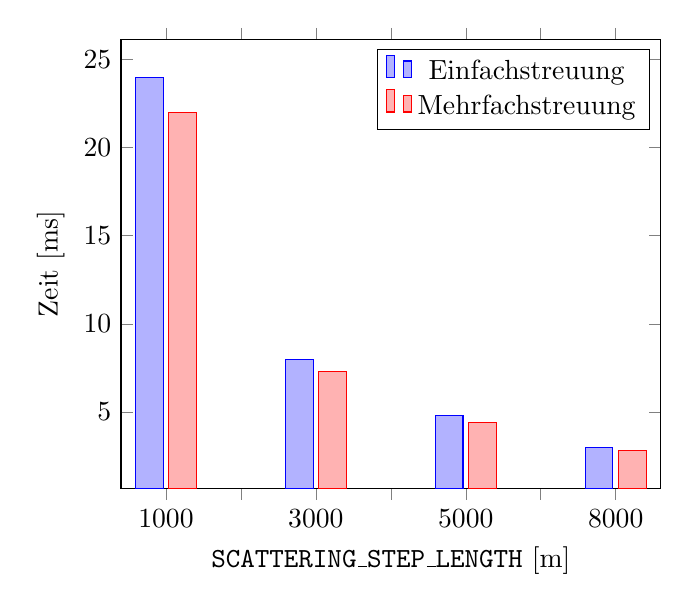
\begin{tikzpicture}
\begin{axis} [
	ybar,
	xticklabels = {,1000,,3000,,5000,,8000}, 
	xlabel=\texttt{SCATTERING\_STEP\_LENGTH} {[m]}, 
	ylabel=Zeit {[ms]} ]

	\addplot coordinates {
		(0,24)
		(1,8)
		(2,4.8)
		(3,3)
	};
	\addplot coordinates {
		(0,22)
		(1,7.3)
		(2,4.4)
		(3,2.8)
	};
	\legend{Einfachstreuung, Mehrfachstreuung}
\end{axis}
\end{tikzpicture}

\caption{Einfluss der Schrittlänge auf die Rechenzeit einer Streuungsordnung}
\label{steps}
\end{figure}

\clearpage
\part{Kombination}
Wolken und Atmosphäre können natürlich separat gerendert werden, da aber die Wolken maßgeblich von der Atmosphäre
beeinflusst werden, sollten sie für realistischere Ergebnisse integriert werden.

Im folgenden wird auf das Zusammenspiel von Geometrie, Atmospäre und Wolken eingegangen.
\section{Implementierung}
\subsection{Renderreihenfolge}
In unserem System wird als erstes die Geometrie, danach die Atmosphäre, und dann die Aerial Perspective gerendert. Das
hat mehrere Gründe:
\begin{itemize}
	\item Da die Atmosphäre von der Geometrie verdeckt ist, kann so das Rendern später sowieso nicht sichtbarer Pixel
	verhindert werden.
	\item Das Raytracen der Wolken sollte abgebrochen werden, sobald Geometrie den Blickstrahl schneidet.
	\item Die Farbe der Wolken muss gegebenenfalls mit der der Geometrie und sicherlich mit der der Atmosphäre gemischt
	werden.
	\item Neben Geometrie muss die Aerial Perspective auch auf die Wolken angewendet werden.
\end{itemize}
Hierbei benötigt jedes erzeugte Fragment nur die Ergebnisse vorheriger Renderpasses an der Stelle des Fragments, die
jeweiligen Pipelines können also als Subpasses in einem einzigen Renderpass ausgeführt werden. Daraus folgt, dass unser
System insbesondere auf Hardware die Tiled Renderering umsetzt, effizient ist.

\subsection{Wolken}
In dem Algorithmus der die Wolken zeichnet wird wiederholt das einfallende Sonnen- und Umgebungslicht bestimmt. An
diesen Punkten kann aus den Atmosphärentexturen gelesen werden: Das Sonnenlicht wird mit Transmittance attenuiert, das
Umbegungslicht wird aus der Streuungstextur für die Höhe der Wolke, die Blickrichtung des aktuellen Fragments und die
Sonnenrichtung ausgelesen.

\section{Evaluation}
Hier werden kurz Visuelle Ergebnisse und finale Performance präsentiert.
\subsection{Visuelle Ergebnisse}
Der Look unseres Himmels ist im ganzen Zufriedenstellend (siehe \cref{final}).

\subsection{Performance}
Auf die Performance der einzelnen Komponenten wurde bereits eingegange, hier sei nochmal erwähnt, dass das letztendliche
System auf einer Radeon RX 6700xt mit einer Auflösung von 2560x1440 je nachdem wieviele Pixel in einem Frame von Wolken
eingenommen werden, Frametimes von 1.7ms(keine Wolken)-13.7ms (nur Wolken) erreicht.
